%% This is an example first chapter.  You should put chapter/appendix that you
%% write into a separate file, and add a line \include{yourfilename} to
%% main.tex, where `yourfilename.tex' is the name of the chapter/appendix file.
%% You can process specific files by typing their names in at the 
%% \files=
%% prompt when you run the file main.tex through LaTeX.
\chapter{Introduction}

%% Chapter outline goes here

\section{Motivations for a fiber optic DOCM system}

\label{sec:intro}

The mammilian cochlea is capable of remarkable sensory perception. It can distinguish motions as small as the radius of a hydrogen atom and discriminate between up to 30 frequencies within a single semitone. \cite{ghafarri} However, the mechanics of motion in the inner ear remain poorly understood. The Micromechanics Group at RLE is  analyzing motion in the cochlea in order to more fully understand what gives rise to these remarkable sensory abilities.

\begin{figure}[h!]
  \centering
    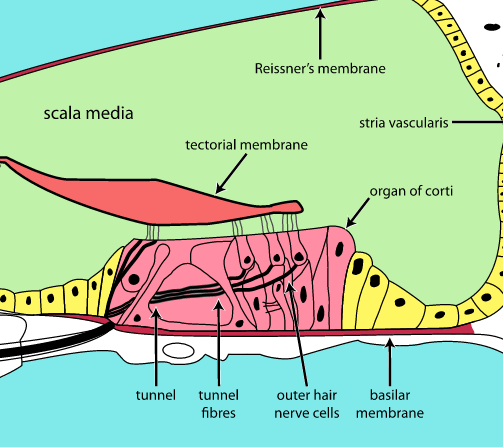
\includegraphics[width=0.8\textwidth]{Images/Background/cochlea.png}
      \caption{A schematic of tissues in the cochlea.}
      \label{fig:cochlea}
\end{figure}

A tissue of particular interest in the cochlea is the tectorial membrane, which is in direct contact with the hair cells, as shown in Figure \ref{fig:cochlea}. This tissue has some interesting mechanical properties, and its position in relation to the sensory cells suggests it could play in active role in motion amplification or in frequency discrimination. However, as it is almost entirely water, it is very difficult to image with conventional imaging techniques.

A technique known as optical coherence tomography allows three-dimensional imaging into tissues, such as the tectorial membrane, by making use of the auto-correlation properties of temporally incoherent light. When used with a high NA lens for high resolution transverse imaging, the technique is also known as optical coherence microscopy. This technique can image deeper into tissues than other three-dimensional imaging methods such as confocal microscopy. Furthermore, OCT allows for measurement of motion (citation here?), both constant and periodic, as will be explained later in the introduction.

The Micromechanics Group at RLE currently uses a doppler optical coherence microscopy, or DOCM (a subset of doppler optical coherence tomography, or DOCT) system to image the mammilian cochlea and acquire data about the mechanical motions of tissues. This system was developed by former student Stanley Hong. \cite{hong}

The current system is designed around free space optics that have been carefully aligned and positioned on an optics table. This design has several disadvantages, chiefly that it is difficult and time consuming to align with the animal that is being imaged. This process can take several hours, due to the need to move the animal precisely under the DOCT objective, and the need to align the cochlea with the fixed optical axis of the DOCT system. Furthermore, the current free space system is bulky and fragile.

The system described in this thesis, while similar in many ways to the existing DOCT system, primarily uses fiber optic coupled components. Fiber optics can be more compact, and are almost insensitive to movement or changes in physical shape (one notable exception to this, with regards to polarization, will be discussed in Chapter 2). Additionally, the objective used for imaging the actual tissue is mounted on a custom designed mechanical apparatus that allows for a variable angle optical axis, and easy repositioning, to work with the researcher and research animal, rather than forcing the animal to conform to the optical system. These improvements should significantly improve the workflow of other researchers in the Micromechanics Group.

\section{Principle of operation of time domain OCT}
\label{sec:principles_oct}

Throughout this document, the coordinate axis parallel to the direction of light emission from the objective shall be referred to as the ``axial'' direction, or ``z'' axis. The plane perpendicular to this axis is known as the ``transverse'' plane, or, sometimes, the ``x'' and ``y'' axes.

\begin{figure}[h!]
\centering
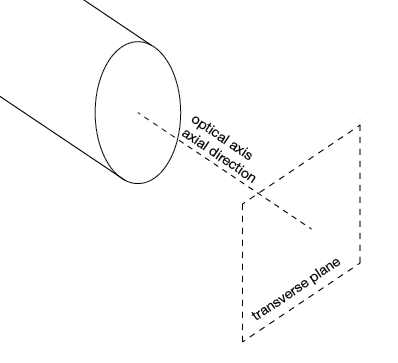
\includegraphics[width=0.6\textwidth]{Images/Background/axes.png}
\caption{Definition of axes.}
\end{figure}

\begin{figure}[h!]
  \centering
    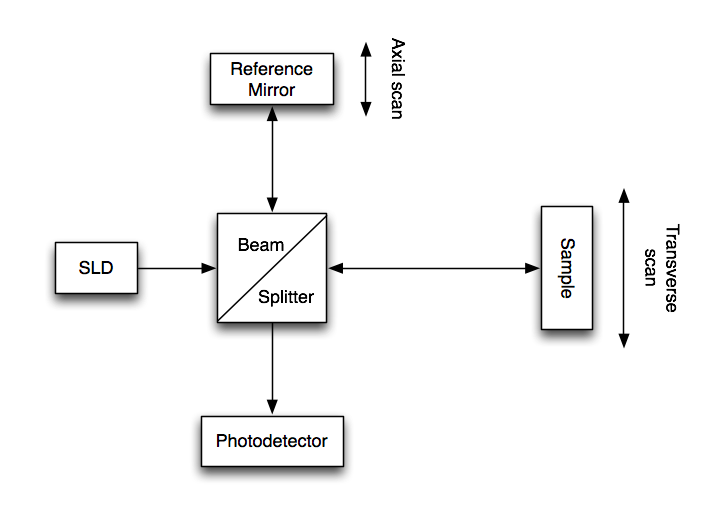
\includegraphics[width=0.8\textwidth]{Images/Background/basic_oct.png}
      \caption{A schematic of a basic OCT system.}
\end{figure}


OCT functions by utilizing the principle of the Michelson interferometer, as shown in Figure 1. Light is split in to two beams. One is reflected from a mirror, the other is scattered from a biological sample. The light is then recombined and the intensity measured by a photodetector. When the optical path lengths of the two beams are closely matched, and interference pattern may be observed. By using temporally incoherent (broadband) light, the interference pattern is capable of absolute localization.

The electric field from a temporally incoherent source can be modeled accurately as a wide-sense stationary random process with a certain power spectral density. \cite{Bouma} In the case where the scattering sample is replaced by a reflecting mirror, the mathematical analysis may be simplified greatly by assuming that two time delayed versions of this processes are being interfered. From this, we show that interference is the same as autocorrelation, and make use of the Wiener-Khinchin theorem. This derivation follows closely that of Fercher et. al. \cite{fercher}

The intensity of light with analytic (complex) amplitude $V(t)$ is defined as:

\begin{equation}
I(t) = V^*(t)V(t)
\end{equation}

In an OCT system, the light from a reference path is combined with the light from a sample path after some delay. We may express this as:

\begin{equation}
V_D(t; \Delta t) = V_S(t) + V_R(t + \Delta t)
\end{equation}

Of course, since measuring instantaneous electric field amplitude is impossible, we are interested in ensemble averages of intensity. This gives the following result, where $\Gamma_{XY}$ represents the cross correlation between two random processes $X$ and $Y$.

\begin{equation}
\begin{aligned}
\bar{I}_E(\Delta t) & =  \langle I_E(t; \Delta t) \rangle \\
& =  \langle V^*_E(t; \Delta t) V_E(t; \Delta t) \rangle \\
& =  \langle I_S(t) \rangle + \langle I_R(t) \rangle + 2 \Re \{\Gamma_{SR} (\Delta t) \}
\end{aligned}
\end{equation}

$\Delta t$ is proportional to the path length difference between the two beams, $\Delta t = \Delta z / c$. When both sample and reference paths are illuminated from the same light source, the cross correlation function above simplifies into an autocorrelation function of the light source. From here, the Wiener-Khinchin theorem can be applied, which states that the autocorrelation function of a wide-sense stationary random process is related to the process power spectral density by a Fourier transform.

\begin{equation}
\Gamma_{XX}(\tau) = 2 \int_{0}^\infty S_{XX}(f) \exp(2 \pi j \tau f) \,df
\end{equation}

Therefore, the axial resolution in an OCT system is limited by the spectral properties of the light source. Given a source of center wavelength $\lambda_0$ and bandwidth $\Delta \lambda$, if we assume a Gaussian PSD, we may find the width of the autocorrelation function, and therefore the axial resolution. \cite{fercher}

\begin{equation} \label{eq:ares}
\delta_z = l_c = \frac{2 \ln{2}}{\pi} \frac{\lambda_0^2}{\Delta \lambda}
\end{equation}

This however, is just the envelope of the autocorrelation function. It is also modulated by a carrier, with a  frequency dependent on the wavelength of the light source, $\lambda_0$, and the speed of the scan, $v_s$. \cite{fercher}

\begin{equation} \label{eq:carrier}
f_{mod} = 4 \pi v_s / \lambda_0
\end{equation}

The transverse resolution is the standard diffraction limit for a lens. \cite{hecht}

\begin{equation} \label{eq:tres}
\delta_x = 0.61 \frac{\lambda}{NA}
\end{equation}

\section{Heterodyne OCT with Acousto-optic Modulators}

As derived in the previous section, the frequency of the carrier is dependent on the speed of the z-axis motion. For typical cases, this is on the order of 1 KHz. If the speed of the scan is variable, this carrier is inconsistent, and if the scan stops at a particular point, the frequency is near zero (non-zero only due to mechanical vibration).

In some cases, it is desirable to have a higher carrier frequency, or a carrier frequency that is independent of the speed of the z-axis scan. This can also be useful for cases where the z speed is zero, as in \begin{em}en-face\end{em} OCT. \cite{bouma}

\subsection{Principle of operation of acousto optic modulators}

\begin{figure}[h!]
\centering
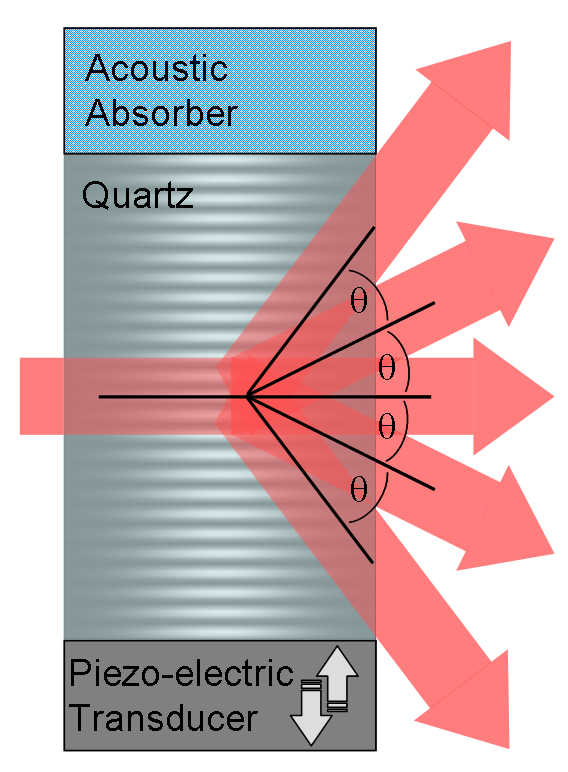
\includegraphics[width=0.3\textwidth]{Images/Background/aom.png}
\caption{Light scatters off of acoustic waves in a quartz crystal, changing both frequency and angle.}
\end{figure}

Acousto optic modulators (AOMs) are crystals, typically quartz, that use acousto-optic effect to shift the frequency of light. A transducer establishes an acoustic standing wave at RF frequencies inside the crystal. Compression waves in the crystal can be modeled as gradients in the refractive index. [McCarron] Light incident upon these refractive index gradients will be scattered.

\begin{figure}[h!]
\centering
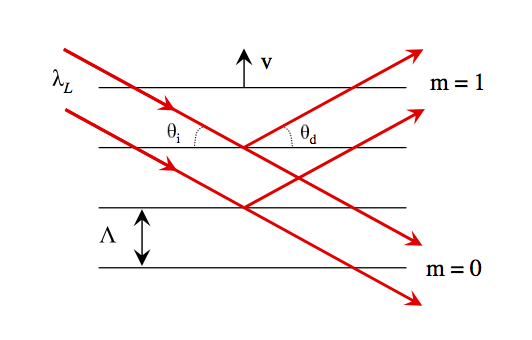
\includegraphics[width=0.5\textwidth]{Images/Background/aom_scattering.png}
\caption{Light scattering off of acoustic wavefronts in an acousto-optic modulator.}
\end{figure}

Scattered light interferes constructively when the following condition is met.

\begin{equation} \label{eq:constructive_interference}
n \lambda_L = \Lambda (\sin{\theta_i} + \sin{\theta_d})
\end{equation}

Conservation of momentum requires that $\theta_i = \theta_d$, which simplifies the constructive interference condition to:

\begin{equation}
n \lambda_L = 2 \Lambda \sin{\theta_d}
\end{equation}


This Bragg diffraction also shifts the frequency of the light up by $mF$, where $m$ is the order of diffraction, and $F$ is the acoustic wave frequency.

In a fiber-coupled AOM, the input and output fibers are aligned with the first order diffraction beam.

\subsection{Generating a carrier wave with AOMs}
\label{sec:aom_carrier}

Even with an imprecise or drifting optical frequency, the precise shift frequency induced by an AOM can be used to generate an extremely stable optical interference signal.

The instantaneous complex electric field can be written for two different frequencies can be written as

\begin{align}
E_a(t) & = E_a e^{2 \pi ft j} \\
E_b(t) & = E_b e^{2 \pi (f + F)t j}
\end{align}

The interference between these two fields creates a beat frequency, with the optical frequency amplitude modulated by the slower RF frequency $F$.

\begin{align}
E_a(t) + E_b(t) = & E_a e^{2 \pi ftj} + E_b e^{2 \pi (f + F)t j} \\
= & E_a e^{2 \pi ft j} + E_b (e^{2 \pi ftj} e^{2 \pi Ftj}) \\
= & e^{2 \pi ftj} (E_a + E_b e^{2 \pi Ftj}) \\
= & E_a(t) (1 + \frac{E_a}{E_b} e^{2 \pi Ftj})
\end{align}

The RF frequency $F$ used to drive the AOMs is typically on the order of 40-200 MHz. For many applications, this is a higher carrier frequency than desired. In this case, it is possible to use two AOMs to generate an even lower frequency carrier, by driving them at slightly different RF frequencies.

\begin{align}
E_a(t) & = E_a \exp{(2 \pi t j (f + F_1))} \\
E_b(t) & = E_b \exp{(2 \pi t j (f + F_2))}
\end{align}

It can be seen via an identical simplification to the above that the combination of these electric field amplitudes creates a carrier wave with frequency equal to the absolute value of $F_1 - F_2$.

\section{Doppler OCT with AOMs}
\label{sec:doppler_aom}

Scattering off of moving particles induces a change in the frequency of scattered light.

%% more equations/background

Excitations and movements of interest are typically sinusoidal in the applications of this OCT device. The instaneous velocity of the scattering media can therefore be written as follows, where $A_o$ is the amplitude of motion and $\omega$ is the acoustic frequency of excitation.

\begin{equation} \label{eq:media_v}
v(t) = A_o \cos{(\omega t)}
\end{equation}

This produces a frequency shift.

%% more equations / background

The new instantaneous electric field amplitudes may be written as follows, and their sum may be calculated.

\begin{align}
E_a(t) & = E_a \exp{(2 \pi t j (f + F_1)(1 + \frac{A_o\cos{\omega t}}{c}))} \\
E_b(t) & = E_b \exp{(2 \pi t j (f + F_2))}
\end{align}

\begin{dmath}
E_b(t) + E_a(t) = E_a \exp{(2 \pi t j (f + F_1))}\left(\exp{\left(\frac{2 \pi t j A_o \cos{wt}}{c}(f + F_1)\right)} + \frac{E_b}{E_a} \exp{(2 \pi t j (F_2 - F_1))}\right)
\end{dmath}

This equation can be simplified slightly by substituting two new symbols for the modified optical frequency and RF frequency difference.

\begin{align*}
f' = & f + F_1 \\
\Delta F = & F_2 - F_1
\end{align*}

\begin{dmath}
E_b(t) + E_a(t) = E_a \exp{(2 \pi t j f')}\left(\exp{\left(2 \pi t j f' \frac{ A_o \cos{wt}}{c}\right)} + \frac{E_b}{E_a} \exp{(2 \pi t j \Delta F)}\right)
\end{dmath}

The instantaneous light intensity is equivalent to the absolute value of the instaneous electric field amplitude squared.

\begin{dmath}
I(t) = E_a^2 \left(1 + \frac{E_b^2}{E_a^2} + 2 \frac{E_b}{E_a} \cos{\left(2 \pi t \left(\Delta F + f' \left( \frac{A_o \cos{\omega t}}{c} \right) \right)\right)} \right)
\end{dmath}

\begin{dmath}
I(t) = E_a^2 + E_b^2 + 2 E_b E_a \cos{\left(2 \pi t \left(\Delta F + f' \left( \frac{A_o \cos{\omega t}}{c} \right)  \right)\right)}
\end{dmath}

The frequency shift induced by the motion of the media can clearly be seen in the instaneous phase of the intensity oscillation.

\begin{dmath}
\label{eq:phase_aom_doppler}
\phi(t) = 2 \pi t \left(\Delta F + f' \left( \frac{A_o \cos{\omega t}}{c} \right)   \right)
\end{dmath}

This is equivalent to frequency modulation, with the periodic change in frequency of:

\begin{equation}
f' \left( \frac{A_o \cos{\omega t}}{c} \right)
\end{equation}

This oscillation can be extracted from the captured signal using the Hilbert transform, as discussed in Section \ref{sec:sigproc_mo_anal}.

\section{Signal processing}

%% signal processing figure

\begin{figure}[h!]
  \centering
\begin{tikzpicture}[node distance = 2cm, auto]
    % Place nodes
    \node [block] (bpf) {Analog band pass filter and preamplifier};
    \node [block, left of=bpf, node distance=3cm] (pd) {Photodiode};
    \node [block, right of=bpf, node distance=3cm] (adc) {Analog to digital converter};
    \node [block, below of=adc, node distance=3cm] (dbpf) {Digital band pass filter};
    \node [block, right of=dbpf, node distance=3cm] (hilb) {Hilbert transform envelope extraction};
    \node [block, right of=hilb, node distance=3cm] (ds) {Downsampling};
    % Draw edges
    \path [line] (pd) -- (bpf);
    \path [line] (bpf) -- (adc);
    \path [line] (adc) -- (dbpf);
    \path [line] (dbpf) -- (hilb);
    \path [line] (hilb) -- (ds);
\end{tikzpicture}
\caption{Basic OCT signal processing chain. The bandpass filter is centered around the carrier frequency from equation \ref{eq:carrier}. The demodulator either can be as straightforward as an envelope follower or a Hilbert transform based analytic continuation.}
\end{figure}

Prior to analog-to-digital conversion, analog bandpass filters select for the carrier frequency and its sidebands.

The Hilbert transform can be used to extract the envelope from the carrier. Given a signal of the form

\begin{equation}
x(t) = A(t)\cos{(\omega t)}
\end{equation}

the Hilbert transform can generate the quadrature component, given by

\begin{equation}
H(x(t)) \approx A(t) \sin{(\omega t)}
\end{equation}

It can therefore be seen that the envelope component of the signal can be calculated quite easily.

\begin{equation}
A(t) \approx \sqrt{(x(t))^2 + H(x(t))^2}
\end{equation}

The envelope, which does need the high sampling rate previously required in order to capture the carrier frequency, can then be downsampled to the resolution required by the imaging application.

\subsection{Analyzing motion}
\label{sec:sigproc_mo_anal}

%As the reference signal $V_{ref}$ is at exactly half the frequency of the captured heterodyne signal $V_{het}$, the following equation gives the instantaneous difference in phase.

As we showed in Section \ref{sec:doppler_aom}, the phase of the amplitude of light scattered off of media moving periodically, which we will refer to as the heterodyne signal, $V_{\mathrm{het}}$, can be expressed as follows.

\begin{equation}
\phi_{\mathrm{het}}(t) = 2 \pi t \left(\Delta F + f' \left( \frac{A_o \cos{\omega t}}{c} \right)   \right) + \phi_{\mathrm{offset}}
\end{equation}

We also must capture a reference signal, notated as $V_{\mathrm{ref}}$, which is the difference between the two RF drive frequencies. This frequency difference is exactly half the carrier frequency of the heterodyne signal, so its phase may be written as:

\begin{equation}
\phi_{\mathrm{ref}}(t) = 2 \pi t \frac{\Delta F}{2}
\end{equation}

The instantaneous phase of an arbitrary signal may be estimated as follows, where $H$ is the Hilbert transform also discussed in Section \ref{sec:aom_carrier}.

\begin{equation}
\phi(t) = \tan^{-1} \left( \frac{H(x)(t)}{x(t)} \right)
\end{equation}

Therefore, the instantaneous phase difference between the heterodyne signal and the reference signal may be written as:

\begin{equation}
\phi(t) = \tan^{-1}\left( \frac{H(V_{\mathrm{het}})(t)}{V_{\mathrm{het}}(t)} \right) - 2\tan^{-1}\left( \frac{H(V_{\mathrm{ref}})(t)}{V_{\mathrm{ref}}(t)} \right)
\end{equation}

Substituting in from Equation \ref{eq:phase_aom_doppler}, with $c$ replaced by $c/n$ to account for the refractive index of the media.

\begin{equation}
\phi_{\mathrm{het}}(t) - 2 \phi_{\mathrm{ref}}(t) = 2 \pi t f'  \left( \frac{A_o \cos{\omega t}}{c/n} \right) + \phi_{\mathrm{offset}}
\end{equation}

Because the RF frequency $F_1 << f$, the optical frequency, we can approximate $f' = f + F_1 \approx f$, and simplify the equation above. The equation can be made simpler still by simplifying to a wavenumber.

\begin{equation}
2 \pi t f'  \left( \frac{A_o \cos{\omega t}}{c/n} \right) + \phi_{\mathrm{offset}} \approx k n A_o \cos{\omega t} + \phi_{\mathrm{offset}}
\end{equation}

The constant offset term may be subtracted off, and consequently the displacement of the sample, $D(t)$ may be calculated.

% ??? Where does Stan's factor of two come from?

\begin{equation}
D(t) = \frac{1}{kn} \phi(t)
\end{equation}

\section{Literature review}

As mentioned in Section \ref{sec:intro}, much of this research is an textension of work done by Stanley Hong, also in the Cochlear Mechanics Group at MIT. In a 2006 paper in the Journal of Biomedical Optics, Hong discussed the first iteration of this time domain doppler OCT system. \cite{hong}

From an optical perspective, there are other researchers that have used GRIN lens optics as an endoscopic objective lens, for instance T. Xie et. al. in 2006. \cite{Xie2006}

%Why time domain? This differentiates our work? Can I spin it positively?

Some work has been done, for instance by H. Subhash et. al. in the field of spectral domain doppler OCT. \cite{Subhash2012} In order to detect motion, the system must be sensitive to changes in optical phase. This is unlike the system described in this thesis, which may be constructed from standard single mode optical fibers, despite the randomization of phase that they create. Unfortunately, Subhash et. al. did not provide sensitivity results to compare against, but it is theorized that a time domain approach can result in higher resolution motion measurements, though at the considerable expense of requiring physical motion to scan the z-axis.

Also Choudhury \cite{Choudhury2011}

This work also continues the active effort of minimizing the size of OCT apparatus, for example the work of B. Goldberg et. al. in the creation of a miniature swept frequency laser source for OCT imaging. \cite{Goldberg2009}

Also of interest in the development of this system, and still a developing field, is the use of algorithms and more sophisticated signal processing to improve the image quality and resolution ability of captured OCT data. Of significant interest is the possibility of correcting for dispersive effects caused by the propogation of light through the sample media. \cite{Xie2005} \cite{DrexlerBook}